\documentclass[12pt,a4paper,oneside,oldfontcommands]{memoir}
\usepackage[utf8]{inputenc}
\usepackage[T1]{fontenc}
\usepackage{microtype}
\usepackage[dvips]{graphicx}
\usepackage{xcolor}
\usepackage{times}
\usepackage[super]{nth}
\usepackage{float}
\usepackage{subcaption}
\usepackage{multirow}
\usepackage[
breaklinks=true,colorlinks=true,
%linkcolor=blue,urlcolor=blue,citecolor=blue,% PDF VIEW
linkcolor=black,urlcolor=black,citecolor=blue,% PRINT
bookmarks=true,bookmarksopenlevel=2]{hyperref}

\usepackage{geometry}
% PDF VIEW
\geometry{total={210mm,297mm},
left=25mm,right=25mm,%
bindingoffset=0mm, top=25mm,bottom=25mm}
% PRINT
% \geometry{total={210mm,297mm},
% left=20mm,right=20mm,
% bindingoffset=10mm, top=25mm,bottom=25mm}
\OnehalfSpacing
%\linespread{1.3}

%%% CHAPTER'S STYLE
% \chapterstyle{bianchi}
\chapterstyle{ger}
% \chapterstyle{madsen}
% \chapterstyle{ell}
%%% STYLE OF SECTIONS, SUBSECTIONS, AND SUBSUBSECTIONS
\setsecheadstyle{\Large\bfseries\sffamily\raggedright}
\setsubsecheadstyle{\large\bfseries\sffamily\raggedright}
\setsubsubsecheadstyle{\bfseries\sffamily\raggedright}


%%% STYLE OF PAGES NUMBERING
%\pagestyle{companion}\nouppercaseheads 
% \pagestyle{headings}
%\pagestyle{Ruled}
\pagestyle{plain}
\makepagestyle{plain}
\makeevenfoot{plain}{\thepage}{}{}
\makeoddfoot{plain}{}{}{\thepage}
\makeevenhead{plain}{}{}{}
\makeoddhead{plain}{}{}{}


\maxsecnumdepth{subsubsection} % chapters, sections, and subsections are numbered
\maxtocdepth{subsubsection} % chapters, sections, and subsections are in the Table of Contents

% \renewcommand{\baselinestretch}{2.0}

%%%---%%%---%%%---%%%---%%%---%%%---%%%---%%%---%%%---%%%---%%%---%%%---%%%

\begin{document}

%%%---%%%---%%%---%%%---%%%---%%%---%%%---%%%---%%%---%%%---%%%---%%%---%%%
%   TITLE PAGE
%
%   due to variety of title page schemes it is probably better to make titlepage manually
%
%%%---%%%---%%%---%%%---%%%---%%%---%%%---%%%---%%%---%%%---%%%---%%%---%%%
\thispagestyle{empty}

\begin{page}

\newcommand{\HRule}{\rule{\linewidth}{0.5mm}} % Defines a new command for the horizontal lines, change thickness here

\center % Center everything on the page
 
%----------------------------------------------------------------------------------------
%	HEADING SECTIONS
%----------------------------------------------------------------------------------------

\textsc{\LARGE University College Cork}\\[1.5cm] % Name of your university/college
\textsc{\Large BSc Computer Science}\\[0.5cm] % Major heading such as course name
\textsc{\large Final Year Project}\\[0.5cm] % Minor heading such as course title

%----------------------------------------------------------------------------------------
%	TITLE SECTION
%----------------------------------------------------------------------------------------

\HRule \\[0.4cm]
{ \huge \bfseries A Deep Learning Regression Model to Predict Galaxy Types Using The Galaxy Zoo GZ2 Data Set
}\\[0.4cm] % Title of your document
\HRule \\[1cm]
 
%----------------------------------------------------------------------------------------
%	AUTHOR SECTION
%----------------------------------------------------------------------------------------

\begin{minipage}{0.4\textwidth}
\begin{flushleft} \large
\emph{Author:}\\
Hassan \textsc{Baker} % Your name
\end{flushleft}
\end{minipage}
~
\begin{minipage}{0.4\textwidth}
\begin{flushright} \large
\emph{Supervisor:} \\
Dr. Gregory \textsc{Provan} % Supervisor's Name
\end{flushright}
\end{minipage}\\[1cm]

% If you don't want a supervisor, uncomment the two lines below and remove the section above
%\Large \emph{Author:}\\
%John \textsc{Smith}\\[3cm] % Your name

%----------------------------------------------------------------------------------------
%	DATE SECTION
%----------------------------------------------------------------------------------------

{\large \today}\\[2cm] % Date, change the \today to a set date if you want to be precise

%----------------------------------------------------------------------------------------
%	LOGO SECTION
%----------------------------------------------------------------------------------------

\includegraphics[width=4cm]{images/ucc.jpeg}
%----------------------------------------------------------------------------------------

\vfill % Fill the rest of the page with white space

\end{page}


\cleardoublepage
%%%---%%%---%%%---%%%---%%%---%%%---%%%---%%%---%%%---%%%---%%%---%%%---%%%
%%%---%%%---%%%---%%%---%%%---%%%---%%%---%%%---%%%---%%%---%%%---%%%---%%%

\tableofcontents*{\listfigurename}
\listoffigures


\clearpage

%%%---%%%---%%%---%%%---%%%---%%%---%%%---%%%---%%%---%%%---%%%---%%%---%%%
%%%---%%%---%%%---%%%---%%%---%%%---%%%---%%%---%%%---%%%---%%%---%%%---%%%


\begin{abstract}
\addcontentsline{toc}{chapter}{abstract}

\Large
 \begin{center}
A Deep Learning Regression Model to Predict Galaxy Types Using The Galaxy Zoo GZ2 Data Set\\ 

\hspace{10pt}

% Author names and affiliations
\large
Hassan Baker
% Hassan Baker$^1$

\hspace{10pt}

\small  
% $^1$) First affiliation\\
% arthur.author@correspondence.email.com\\
% $^2$) Second affiliation

\end{center}

\hspace{10pt}

\normalsize
This project studies various aspects of deep learning, by using empirical comparisons. This involves a study of three learning optimization algorithms; Stochastic Gradient Descent (SGD), SGD with Nesterov momentum, and Adam. This is done across various learning rates to find an optimal combination. Furthermore, this project studies activation function selection, comparing Sigmoid to ReLu, and ReLu to Maxout finding that a Maxout-Sigmoid combination performs far greater for this particular data set. These studies are accomplished by building a deep convolutional neural network to form a regression model using TensorFlow. This study uses the Kaggle Galaxy Zoo Challenge \textit{GZ2} data set, containing images of galaxies, and probability distribution solutions.

% \vspace*{\fill}
% \paragraph{}
% Abstract
% \paragraph{}
%     \textbf{}
% \vspace*{\fill}

\end{abstract}

\chapter{Introduction}

\section{Galaxy Zoo}
Galaxy Zoo is one of the world’s largest citizen science projects in the world. The project collects images of galaxies and invites the public to classify the images into set classes. The classification process is done by giving the citizens a set of questions to answer regarding the morphology of the galaxies in the images.  The public's assessment of the data is later aggregated and cleaned. The project managed to get more than 50 million classifications in its first year using images of galaxies taken from the Sloan Digital Sky Survey (SDSS). 

Galaxy Zoo 2 (GZ2) refers to the second phase of the project. The images in the \textit{GZ2} data set compromise of the brightest 25\% from the SDSS~\cite{Willett}. This dataset contains more than 300,000 images. The public was asked to classify the galaxies in the images into 11 classes, which contain sub classes. This accumulates to 37 possible classes altogether. The galaxies were classified by the public’s answering of questions like “Is the galaxy smooth and rounded, with no sign of a disk?” These questions form a decision tree of 37 possibilities, which are the labels of the dataset. 

    \begin{figure}[ht]
    \center
      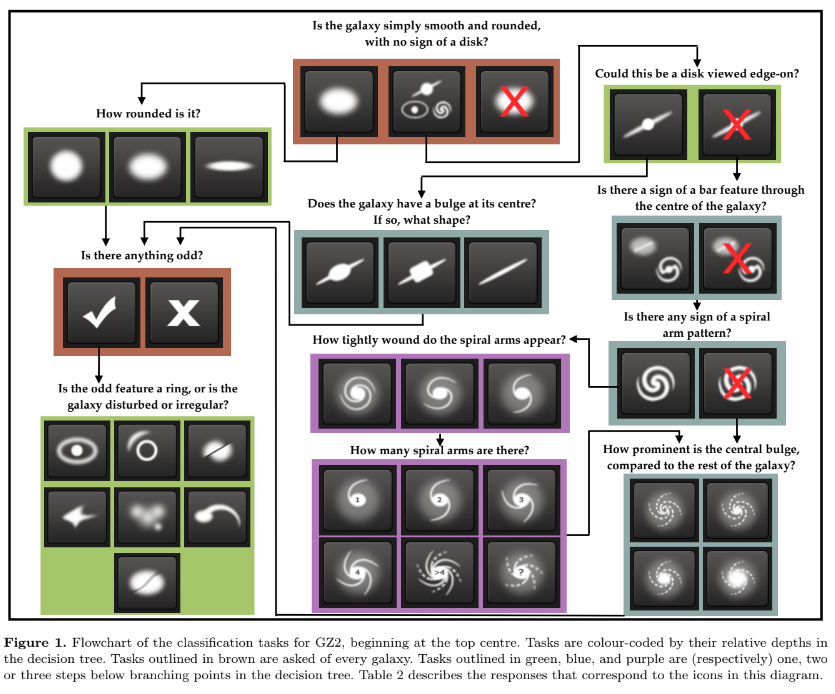
\includegraphics[width=\linewidth]{images/gz-2-decision-tree.png}
      \caption{Decision tree of galaxy labels in the GZ2 data set taken from Willett et al~\cite{Willett}.}
      \label{fig:GZ2-Decision-Tree}
    \end{figure}

\section{The Galaxy Challenge}

The Galaxy Zoo Galaxy Challenge was launched on the \nth{20} of December 2013 and hosted on Kaggle. The competition provided the set of \textit{GZ2} data. A set of probability distributions relating to what class the public judges each image to belong to is also given as a CSV files. The objective of the competition is to reproduce similar probability distributions for a test set. The majority of the solutions produced for this competition involved machine learning, and a majority of that majority relied heavily on convolutional neural networks.

Given the large set of image data, convolutional neural networks are an obvious choice as their use is proven to be highly effective in image recognition and analysis. However, convolutional neural network solutions, like many machine learning solutions, contain a level of complexity that originate from just how varying the model can be. One can refine at each step of the process to yield better accuracy or lower error, but in many ways, one can also over refine.

\section{Neural Networks}
Neural Networks are constructed by layers that consist of parrallel neurons which contain weights and biases. The data is inputed into the first layer. At each neuron, the input is multiplied by the weight, and the bias is added to the solution.  The output of each neuron is then put through a non-linear function. This is so as to introduce non-linearity in the network, as most data forms around non-linear models, which would mean a linear model would not fit. Each output is then passed into the folowing layer, abiding by the connection scheme i.e. in a fully connected network, each neuron passes it's output to every other neuron in the following layer. 

The final layer in a neural network outputs the predictions, given an input. So as to give accurate predictions, the network is trained. Training involves putting a set of training inputs through the network, and measuring the difference between what the network predicts and what the actual values it should predict are, this is known as the loss. The loss is minimised throughout each training iteration using the backpropagation algorithm. ... backprop define + ref



\section{Convolutional Neural Networks}

Convolutional neural networks methods are used widely for image recognition, sound recognition, natural language processing~\cite{Bhandare}, and a whole cohort of other applications.

Convolutional neural networks are currently one of the most popular machine learning techniques. They are powerful machine learning methods as they rely on breaking down the image into smaller convolutions and detects whether the learned patterns exist in these convolutions. The order and location of where these patterns occur is less important than in an ordinary feed-forward neural network, which is actually beneficial for particular tasks, such as image recognition.

Convolutional neural networks are more efficient to train and need less data than regular feed-forward networks, even though their theoretical maximum accuracy is not as good. This is because the convolutional layers that make them quicker to train than standard neural networks. These layers convolute the data into separate learning phases. An earlier layer would tend to take on the job of edge detection, and pass that information to the following layer. As you move through the layers, the learned filter should get more complex, until it eventually recognizes whole objects. This is because each individual layer can be seen as a separate network which is optimized, through training, to produce the easiest solution for the following layer to work with. 

This feature of convolutional neural networks allows for useful methods like transfer learning, whereby one can take the convolutional layers of one already trained network, attach a new fully connected layer to it, and train it to recognize something else entirely, far quicker than it would to train a whole new network.

% \subsection{Second subsection}

\chapter{Analysis}



\section{Goals}

The main goal of this project is to develop a robust convolutional neural network that can produce a probability distribution for the test set with a low level of error, using Root Mean Squared Error (RMSE) for error estimation.

This model will be built incrementally by creating an initial model, and using it to study some key components of deep learning methods and architecture. Taking the results of these studies, the model will be improved to produce more optimal models. As the data is from a Kaggle competition from four years ago, there are already solutions available on the internet. The solutions examined in this study are Team 6789~\cite{Nguyen}, Fang-Chieh Chou~\cite{Fang}, and most notably Sander Dieleman~\cite{Sanders-GZ}. Hence this project focuses on studying some of the methods used in those solutions, as well as alternatives put forward by the student.

One of the key areas of study in this project will focus on data preparation and processing, deep learning optimization algorithms, activation function comparisons, and learning rate searching.

One of the studies in this project will aim to validate what the most fitting learning optimization algorithm to use, comparing Stochastic Gradient Descent (SGD), SGD with Nesterov Momentum, and Adam Optimization. This project will also study the effects of using the ReLu function against the use of the Sigmoid function in the final layer of the network. This project also aims to study the effects of the Maxout unit, described in Goodfellow et al~\cite{maxout}, as well as how it can be used in conjunction with the dropout regularization method.

As a tangential goal, the student has undertaken this project to further their knowledge in deep learning methods and principles in a practical sense.

\section{Tools}

(Nothing here yet)

\section{The Data}

The \textit{GZ2} dataset consists of 61,578 training images, 79,975 test images, a CSV file consisting of the 37 probability distributions for each example in the training set, as well as CSV files containing all one ones, all zeros and central pixel benchmarks for comparison when training. The test set solutions are not provided, instead one is required to generate a CSV file with their own solutions and submit them. Seeing this is a large dataset, \textit{holdout} validation was used instead of \textit{k-fold}, as \textit{k-fold} would otherwise be far too time consuming. A validation set was created from 10\% of the training set. This 10\% portion was moved into its own directory and was not used for analysis or training. This allowed for \textit{holdout} validation throughout analysis and training.


    \begin{figure}[ht]
    \center
      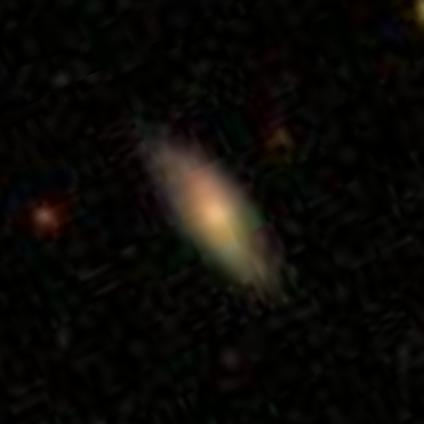
\includegraphics[width=7cm]{images/100023.jpg}
      \caption{An image of a galaxy from the GZ2 data set.}
      \label{fig:GZ2-1}
    \end{figure}
      

\subsection{Cropping} \label{Cropping}

The images in \textit{GZ2} are already centered and are \(424\times424\) in size. It does not seem feasible to fit every pixel of an example as a feature into the network as that would result in an input layer of shape \([424, 424, 3]\). This is far too big and would slow down learning greatly. The galaxies in the images are surrounded with black space. Sometimes these images contain some other stellar objects that have no apparent significance for the model. The black space and the stellar objects make for plenty of noise. Therefore it is only reasonable to uniformly crop these images so as to cut off a majority of the noise but still keep every galaxy intact. 

The winning solution, Sander Dieleman~\cite{Sanders-GZ} cropped the images to a standard size of \(207\times207\). However, there is no indication as to how the value \(207\times207\) was selected in this solution. 

To investigate this, using a Python script, all the images in the training set were analysed to validate this crop amount. The most important and active parts of the image are at the centre, accounting for most of the brightness in each image. Whereas the more dim areas are more likely to contain noise. Using brightness as a measure of activity, we can measure how much we have to crop each image to keep a selected threshold \(k\) of activity, \(k\) being the percentage of brightness in an image. Hence, each image’s colour channels are normalized to fit a the range \(0 < i < 1\), and are averaged into 1 channel (gray-scale).

Each individual image is then iteratively cropped towards the centre. In each iteration a 1 pixel wide perimeter was cropped out of the image. \(k'\), the percentage of brightness of an image was taken at each iteration. Once \(k'\) falls below \(k\), the amount of iterations carried out for that particular image are appended to a list \(Z\).

Once the whole training set is analysed, the mean of the values in \(Z\) is taken. Using trivial geometry, one can then determine the optimal crop amount for a mean of \(k\) brightness in the images. The mean value of \(z\), denoted by \(z\) amounts to how many pixels down the diagonal of the image to crop from. Given the value \(H\), the length of the diagonal from one corner of the original image to the opposite corner. This means that the length of the diagonal from one corner to the opposite corner of a cropped image, \(h\) is found using \(h = H - 2z\). Furthermore, seeing as the crop results in square dimensions, taking the dimension values as \((x, x)\), \(x\) can be found using Pythagoras. 

In this analysis, \(k\) was selected to be 90\%. This yielded a mean crop amount of \(218\times218\), which is only \(11\times11\) more than the \(207\times207\) amount selected in Dieleman's solution~\cite{Sanders-GZ}, and \(18\times18\) more than the \(200\times200\) amount used by Team 6789~\cite{Nguyen}. Which leads to a conclusion that the crop amount in these solutions was either selected with good intuition, which is very possible, or else selected in a similar fashion with an extra few pixels kept for extra measure so as to make sure that outliers do not impact the results. To verify this, along with the mean crop amount, the maximum and minimum crop amounts for \(k=90\%\) were also taken. The maximum crop amount was \(398\times398\), and the minimum was a crop amount of \(0\times0\). It is easy to see how the minimum and maximum could skew this investigation by just looking at the image itself.  

\begin{figure}[H]
  \centering
  \begin{subfigure}[b]{0.4\linewidth}
    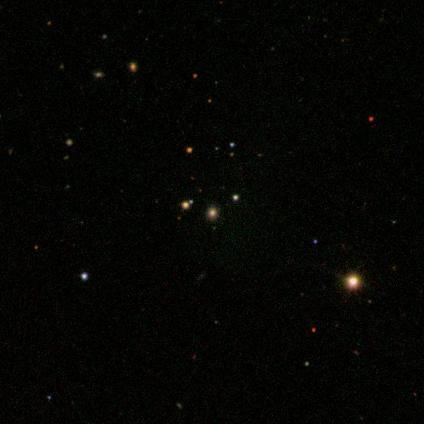
\includegraphics[width=\linewidth]{images/maximum-256411.jpg}
    \caption{The image requiring maximum crop, because the galaxy is very small and is easily confused with other stellar objects.}
  \end{subfigure}\hspace{1cm}
  \begin{subfigure}[b]{0.4\linewidth}
    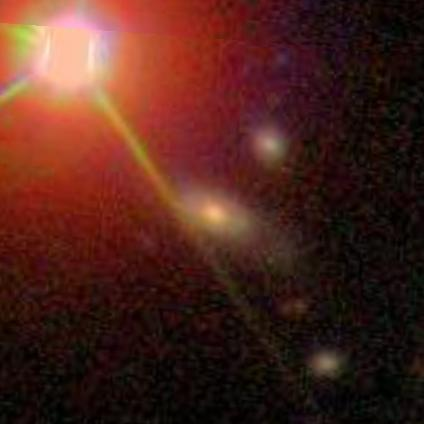
\includegraphics[width=\linewidth]{images/minimum-308196.jpg}
    \caption{The image that requires minimum crop due to the very bright stellar object is in the top right corner.}
  \end{subfigure}
  \caption{Outlier images found in GZ2}
  \label{fig:GZ2-2}
\end{figure}

So as to keep to a middle-ground, and to stick to comparable measure, the crop amount that was selected in this study is \(207\times207\), the same used in Dieleman's solution~\cite{Sanders-GZ}.

\subsection{Down-scaling}

Cropping alone, still results in a very input large size as it would result in an input layer with 128,547 parameters, which will still stagnate the learning time, as all these parameters will have to be updated. Hence, the images were down-scaled by a factor of 1/3, as seen in Dieleman's solution~\cite{Sanders-GZ}. This results in the images taking the shape of \([69, 69, 3]\).

\subsection{Data Augmentation} \label{aug-section}

The images in the \textit{GZ2} data set contain exploitable variances. For instance, as they are images of galaxies, there is no up or down, or left or right. They are of uniform shapes, meaning that it is relatively easy to extract new features out of the given features. 

Inspired by the augmentation section in Dieleman's solution~\cite{Sanders-GZ}, a class for augmenting images was written. This class contains methods for cropping, down-scaling, rotation, and flipping. Uusing this class, one can can augment an image to extract 16 examples out of each individual image.

The augmentation process is thus. The \(207\times207\) crop is applied to each image, a 45 degree rotation of that same image, as well as a horizontal flip of the unaltered image, and the rotated one. This produces four images. This is illustrated in figure \ref{fig:sanders-aug-1}. 

\begin{figure}[H]
  \centering
    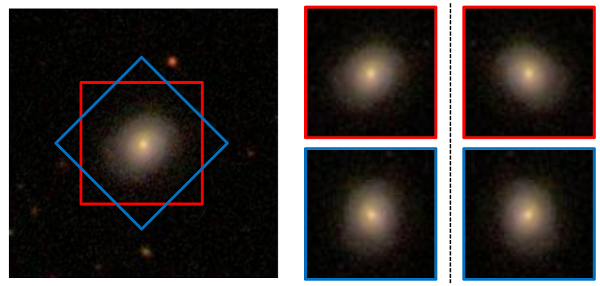
\includegraphics[width=\linewidth]{images/sanders-aug-1.png}
    \caption{Visualization of how 4 features are extracted from one image. Figure taken from Sander Dieleman's blog~\cite{Sanders-GZ}}
    \label{fig:sanders-aug-1}
\end{figure}

Furthermore, four crops of \(45\times45\) overlapping parts are taken from each corner of the images extracted, which produces 16 images in total. The 16 images are then rotated to ensure that all extracted images are oriented so that the galaxy is at the bottom right.


\begin{figure}[H]
  \centering
    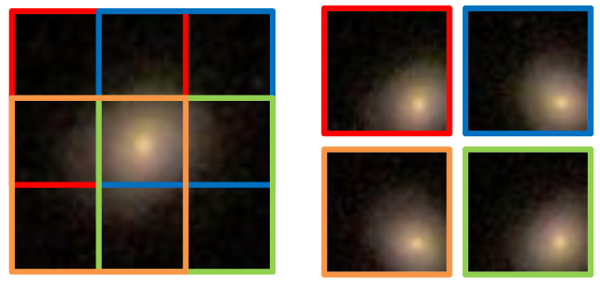
\includegraphics[width=\linewidth]{images/sanders-aug-2.png}
    \caption{Visualization of how the four overlapping parts are extracted from each images created in \ref{fig:sanders-aug-1}. Figure taken from Sander Dieleman's blog~\cite{Sanders-GZ}}
    \label{fig:sanders-aug-2}
\end{figure}

These extracted images overlap by design. This is so as to increase parameter sharing in the model. The bottom right of all extracted images contains the centre of the galaxy, however, the top right contains black space, or noise. Due to this augmentation, the values of the noisy sections are generally different in each extracted image, hence this process makes it more likely for a model to be more active with the bottom right sections.

\chapter{The Network: Tycho1}



The initial convolutional neural network, named Tycho1 is a modified version of the model described in Dieleman's blog ~\cite{Sanders-GZ}. It contains four convolutional layers, and three dense layers. Tycho one differs from Dieleman~\cite{Sanders-GZ} in the dense layers, and does not perform a concatenation on augmented image segments after they have passed the convolutional layers. This is because Tycho1 is designed to train faster, so as to validate the studies regarding learning optimization algorithms, learning rate searching, and activation function comparisons. 

\section{The Architecture}

\begin{figure}[H]
  \centering
    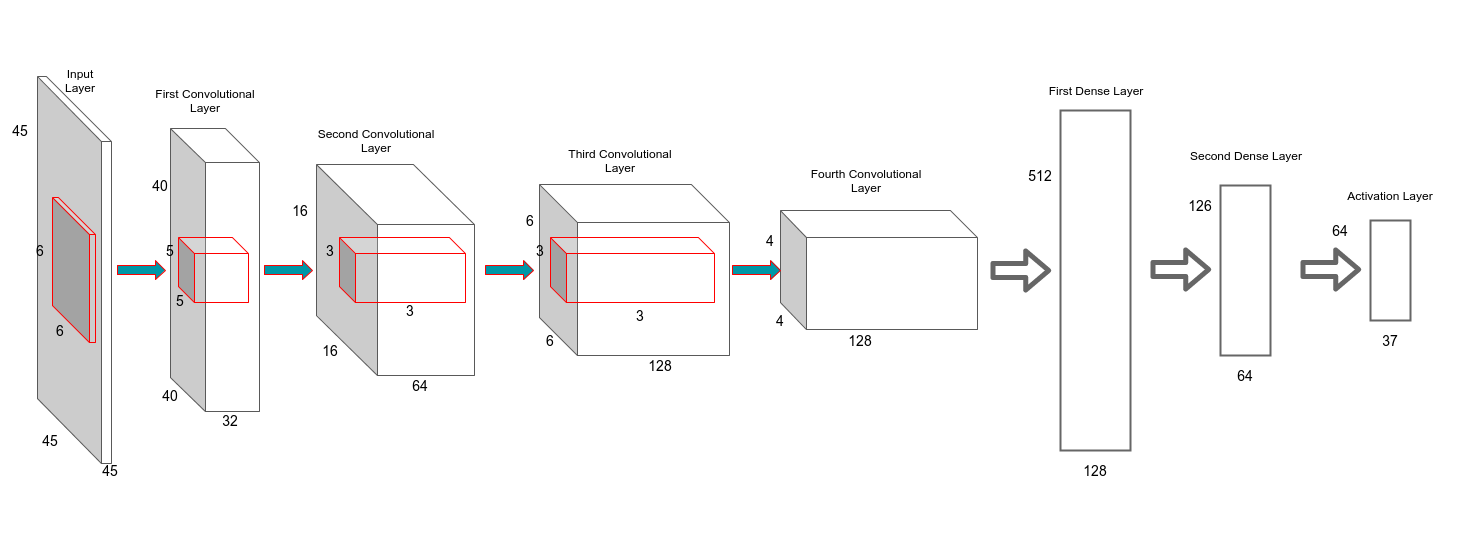
\includegraphics[width=\linewidth]{images/Tycho1.png}
    \caption{Diagram of the Tycho1 network}
    \label{fig:tycho1}
\end{figure}


The input layer takes inputs of shape \([BATCH\_SIZE, 45, 45, 3]\). The first element is the amount of images in a given batch, the second and third represent the size of each image, and the last element is the number of channels. This is then fed into the convolutional segment.

The network consists of four convolutional layers. The first convolutional layer contains a filter of size \(6\), and an output shape of \(32\). The second layer contains a filter of size \(5\) and an output shape of \(64\). The third and fourth both have a filter size of \(3\), and an output size of \(128\). The first, second, and fourth layers are followed by \(2\times2\) max-pooling layers. Once the data passes through the last convolutional layer, it is flattened into a shape of [some shape I can’t remember rn].

The flattened output the enters the dense layers. The weights in the first dense layer and the second dense layer are of shapes \([512, 128]\) and \([128, 64]\), respectively. 

All layers, bar the last contain a Rectified Linear Unit (ReLu) as the activation function.

\begin{equation}
    f(x)=max(x, 0)
    \label{eq:relu}
\end{equation}



The ReLu activation function was chosen as it is extremely useful for object recognition ~\cite{ReLu}. A distinct feature of ReLu activation is that it has sparse activity allowing for mostly meaningful activations to be passed onto the next layer. This decreases training time, and makes activations far more efficient.

The weights in all layers, dense and convolutional, except the last, are initialized to be in a normal distribution of standard deviation \(0.01\), and a mean of \(0\). This restricts the weights to a range of \(-0.01 < W < 0.01\). 

The biases in all layers, including the last, are set to be a constant of \(0.1\). This was originally set to \(0.0\), but after some testing, \(0.0\) proved to be ineffective and resulted in dead units. Hence \(0.1\) is used instead.

The last layer is also a dense layer. This is of shape [BATCH\_SIZE, NUM\_LABELS].This shape corresponds to the amount of images to fed into the network, and the number of values/labels to predict. With this data, there are \(37\) labels.  The weights are initialized to be in a normal distribution of standard deviation \(0.001\), and a mean of \(0\). 

As described by Dieleman ~\cite{Sanders-GZ} and Fang-Chieh ~\cite{Fang}, a modified version of ReLu or Softmax, with a normalization segment was initially considered. However this is where TensorFlow has it's drawbacks, as there is no way to write custom activation functions using the TensorFlow Python API.

As an alternative, Sigmoid activation \ref{eq:sigmoid} is chosen for the last layer. This seems like the best fit as it squashes all values between a range of \(0 < y' < 1\).

\begin{equation}
    h(x) =  \frac{\mathrm{1} }{\mathrm{1} + e^-x }
    \label{eq:sigmoid}
\end{equation}

The error evaluation function used for the Kaggle competition is Root Mean Squared Error (RMSE), hence, for measuring loss, Mean Squared Error (MSE) was used, so as to avoid using the same function for measuring loss and error.

\begin{equation}
     MSE = \frac{1}{n}\Sigma_{i=1}^{n}{({y_i -y'_i})^2}
\end{equation}

\begin{equation}
     RMSE = \sqrt{\frac{1}{n}\Sigma_{i=1}^{n}{({y_i -y'_i})^2}}
\end{equation}

Where \(n\) is the the batch size, or more generally, the number of predicted outputs. \(y\) is the the correct answers given a prediction, and \(y'\) is the predicted output.

\section{Missing Component}
There's a vital missing component in Tycho1 that has been purposely left out. This is the learning optimization algorithm. This will be studied further and decided on in chapter \ref{study}

\section{Data Pre-processing}

What is interesting about the \textit{GZ2} dataset is that the test set contains more examples than the training set. To accommodate for this, the image augmentation described in \ref{aug-section} is used. However, unlike Dieleman's model ~\cite{Sanders-GZ}, the resulting 16 images from the augmentation process we’re not concatenated. Instead, one random image from those 16 generated was selected. This serves to create more inputs to help the model generalize more towards the active parts of each image (bottom right, where the galaxies are), and reduce chances of over-fitting. 

\chapter{Deep Learning Optimizer Algorithms \& Hyper-Parameter Search} \label{study}


A major key to deep learning is the learning optimization algorithm. The model described by Dieleman ~\cite{Sanders-GZ} details the usage of Stochastic Gradient Descent (SGD) of an initial learning rate of \(4\times10^{-2}\), and a Nesterov momentum of \(0.9\). 

However, there are alternatives to this algorithm. Most notably, SGD without Nesterov momentum and Adam optimization. A comparison of these algorithms was made on separate learning rates so as to empirically decide on the most suitable.

\section{Study Description}

[Todo - Add tables and graphs]

The Tycho1 network was set up to take an input of a mini-batch of \(16\) images, that are augmented, with one of the augmented images chosen at random. This model would train for \(2000\) epochs. 

To compare the algorithms, the training was run in a for loop to try out the different algorithms along with four different learning rates \(4\times10^{-2}\), \(4\times10{^-3}\), \(1\times{10^-4}\), and \(1\times10^{-4}\). Throughout these iterations, the loss and error values on both the training set and validation set is taken every 10 epochs. TensorBoard proved to be a vital tool for carrying out this comparison. It made it so that the loss and error values were stored and easily compared by overlaying them through the UI.

\section{Results}

Each algorithm took roughly thirty five minutes to complete one iteration on one learning rate, so the whole comparison took about 7 hours to complete.

It's worth noting that on many occasions the validation error is lower than the training error. This was discovered after the comparison, and is expected to have something to do with the size of the validation set, in comparison to the training set

\subsection{Stochastic Gradient Descent}

Stochastic Gradient Descent performed well on the first learning rate, \(4\times10^{-2}\), producing an RMSE of \(0.1766\) on the training set, and \(0.1969\) on the validation set, on the final epoch. However, when the learning rate was decreased, it performed very poorly, resulting in training and validation RMSE of approximately \(0.45\) for all other learning rates.

\subsection{Stochastic Gradient Descent With Nesterov Momentum}

SGD with Nesterov momentum proved even more effective on the \(4\times10^{-2}\) learning rate, producing a training and validation RMSE of \(0.1766\) and \(0.1725\) on the validation set on the final epoch. However, as the learning rate decreased, the performance decreased too. Interestingly though, the decrease was not as drastic as SGD without Nesterov momentum, as on the \(4\times10{^-3}\), it achieved a training and validation RMSE of \(0.1950\), and \(0.1564\) respectively. This algorithm did however result in error values of about \(0.45\) on the last two learning rates, just as the previous algorithm did.

\subsection{Adam} \label{Adam}

On the first learning rate, the Adam algorithm achieved considerably greater results than other algorithms, producing an RMSE of \(0.1811\) and \(0.1632\) on the training and validation sets respectively on the final epoch, with the learning rate of \(4\times{10^-2}\). This performance did however decrease on the second learning rate of \(4\times10{^-3}\), to being \(0.2304\) and \(0.2482\) for training and validation, respectively. Moreover, on the learning rate of \(4\times{10^-4}\). It did however decrease to a train RMSE of \(0.1517\) and a validation RMSE of \(0.1479\). For the learning rate of \(1\times{10^-4}\) it achieved an RMSE of \(0.1801\), and \(0.1852\) on the training and validation sets respectively. These results showed that the Adam algorithm was far more suitable and stable for this model. 

\subsection{Further Learning Rate Tests On The Adam Algorithm}

From the results of section \ref{Adam}, it looks apparent that lower learning rates perform better, with the exception of the first learning rate of \(4\times{10^-2}\). So in that vain, to smaller learning rates of \(4\times{10^-5}\) and \(4\times{10^-6}\) were tested with the same configuration as the tests above but produced lower RMSE values than it did with a learning rate of \(4\times{10^-4}\).

\begin{figure}[H]
    \centering
    \begin{tabular}{ |c|c|c|c|c| } 
    \hline
    Algorithm & Learning Rate & Training RMSE & Validation RMSE \\
    \hline
    \multirow{4}{4em}{SGD}
    & \(4\times10^{-2}\) & \(0.1766\) & \(0.1969\)\\ 
    & \(4\times10^{-3}\) & \(0.4410\) & \(0.4526\)\\ 
    & \(4\times10^{-4}\) & \(0.4528\) & \(0.4519\)\\ 
    & \(1\times10^{-4}\) & \(0.4472\) & \(0.4528\)\\
    \hline
    \multirow{4}{4em}{Nesterov}
    & \(4\times10^{-2}\) & \(0.1819\) & \(0.1725\)\\ 
    & \(4\times10^{-3}\) & \(0.1950\) & \(0.1564\)\\ 
    & \(4\times10^{-4}\) & \(0.4361\) & \(0.4329\)\\ 
    & \(1\times10^{-4}\) & \(0.4446\) & \(0.4567\)\\
    \hline
    \multirow{4}{4em}{Adam}
    & \(4\times10^{-2}\) & \(0.1811\) & \(0.1632\)\\ 
    & \(4\times10^{-3}\) & \(0.2304\) & \(0.2482\)\\ 
    & \(4\times10^{-4}\) & \(0.1566\) & \(0.1531\)\\ 
    & \(1\times10^{-4}\) & \(0.1801\) & \(0.1852\)\\
    & \(4\times10^{-5}\) & \(0.1632\) & \(0.1824\)\\ 
    & \(4\times10^{-6}\) & \(0.1593\) & \(0.1876\)\\
    \hline
    \end{tabular}
    \caption{The resultant RMSE's for each learning rate on each algorithm}
    \label{fig:learning_rates_table}
\end{figure}

\section{Conclusion} 
As the Adam algorithm performed the best on all learning rates, that will be the chosen algorithm for the models. Furthermore, by looking at the graphs on TensorBoard of all the tests carried out on the Adam algorithm, with a smoothing of \(0.85\), the learning rate of \(4\times{10^-4}\) seemed to be a marginally better choice than \(4\times{10^-2}\), even though it began to converge later, it ended with a lower RMSE. Furthermore also sloped further down than the learning rate of \(4\times{10^-2}\), indicating that it will perform even better if it was run further. Hence the chosen learning rate is \(4\times{10^-4}\).

\chapter{Tycho1 - Evaluation} \label{tycho1}


\section{Training Details}

A training script was written for the Tycho1 model using the Adam Optimizer, on a learning rate of ... The script is set to train on a mini-batch of 256, using the full training set (including the data used in validation for chapter ~\ref{study}), for 10,000 epochs. During the tests in chapter \ref{study}, it was noticed that recording the logging summaries took a substantial amount of time, when compared to training, hence the recording interval is set to 100. This means that the TensorBoard log summary was taken every 100 epochs. A nice side effect of this is smoother graphs.

Taking away more data from the training set for validation does not seem viable here, as the training set itself is already smaller than the test set. Hence, a test interval of 1000 is set, This allows for a CSV of predictions on the test set to be generated ever 1000 epochs so as to accurately assess the rate of change in the model's error, in comparison to the train error, as the validation set proved too small in chapter \ref{study}. 

Unfortunately there was an error in the code, that made it so test conditions were never satisfied. However the status of the model was saved every 100 intervals, meaning allowing the training to be paused and for the script to be altered so as to meet these conditions and produce the test results. Hence we will find that the first few results do not match the test interval. 

As the training surpassed \(10,000\), it becomes apparent that there is still room for improvement, and that training the model further could in fact keep improving the results. Hence, it was allowed to train for another day and a half. In total training took four days, including the time taken to generate the predictions on the test file, which on average took 45 minutes to generate.

Furthermore, as the training started to produce results, it produced some very low values, but no hard \textit{zero's}. This was a known consequence of using Sigmoid activation in the final layer. However, the impact seemed greater as the training went on, as the more training is done the values that should be zero, tend closer to zero, but never get to zero. Hence we see a very drastic retardation in loss and error. So as to test this, the code regarding the custom activation layer from Deleemm ~\cite{Sanders-GZ} was adapted so as to normalize the prediction on the test set. This normalization was practiced when the training reached the \nth{12,000} epoch, and onward from there. 

\section{Results}


\begin{center}
 \begin{tabular}{||c | c | c||} 
 \hline
 Epochs & Training Error & Test Error \\ [0.5ex] 
 \hline\hline
 27102 & 0.1252 & 0.12111\\ 
 \hline
 4001 & 0.1181 & 0.11452\\
 \hline
 6901 & 0.1060 & 0.10968\\
 \hline
 8203 & 0.1020 & 0.10636\\
 \hline
 9004 & 0.1077 & 0.10635\\ 
 \hline
 11005 & 0.1016 & 0.10446\\ 
 \hline
 12000 & 0.1072 & 0.10283\\ 
 \hline
 12000 - Normalized & 0.1072 & 0.10278\\
 \hline
 14700 & 0.1043 & 0.10239\\ 
 \hline
 14700 - Normalized & 0.1043 & 0.10220\\ [1ex] 
 \hline
\end{tabular}
\end{center}

The final RMSE of 0.10220 would rank the Tycho1 model \nth{55} out of the 326 participants in both the private and public leaderboards of the Kaggle Galaxy Zoo competition. This puts it in the bronze ranking, and 5 spots away from a silver ranking. 

\section{Conclusion}

The Tycho1 network does seem to under-fit the data, however not very much, as it has successfully generated a model with what is empirically a good ranking by the competitions standards. However, some issues have come to light from this training.

Normalizing the output, does indeed improve the results, albeit slightly. This makes it apparent that a more suitable activation function is need in the final layer, as although one can normalize the output, the model cannot calculate the gradient for the normalized output on the training set. Hence, it cannot update variable values accordingly to these values. 

Although the Sigmoid activation function does produce decent results, it does hit a limit very quickly, which stagnates
learning greatly.

Allowing the network to run for another day or two would very likely get it in the silver ranking, however, this is not a very effective strategy, as the Tycho1 model does show some heavy signs of retardation when it it comes to loss, and error.

An important conclusion to note, is that the training errors and test errors are reasonably close to each other, indicating that the assumption of the validation set being to small is correct. This means that we can expect validation loss and error to be lower than training loss and error throughout.

\chapter{Tycho2}


So as to decrease 

\section{Validation}

\section{Training Details & Results}

\section{Conclusion}

\chapter{Tycho3}


\section{Validation}

\section{Training Details & Results}

\section{Conclusion}

\chapter{Tycho4}


\section{Validation}

\section{Training Details & Results}

\section{Conclusion}

\chapter{Model Averaging}


\chapter{Project Conclusion}


\chapter{Closing Remarks}



\appendix

\renewcommand{\bibname}{References}
\bibliographystyle{unsrt}
\bibliography{references}

\end{document}

